% (The MIT License)
%
% Copyright (c) 2023 Yegor Bugayenko
%
% Permission is hereby granted, free of charge, to any person obtaining a copy
% of this software and associated documentation files (the 'Software'), to deal
% in the Software without restriction, including without limitation the rights
% to use, copy, modify, merge, publish, distribute, sublicense, and/or sell
% copies of the Software, and to permit persons to whom the Software is
% furnished to do so, subject to the following conditions:
%
% The above copyright notice and this permission notice shall be included in all
% copies or substantial portions of the Software.
%
% THE SOFTWARE IS PROVIDED 'AS IS', WITHOUT WARRANTY OF ANY KIND, EXPRESS OR
% IMPLIED, INCLUDING BUT NOT LIMITED TO THE WARRANTIES OF MERCHANTABILITY,
% FITNESS FOR A PARTICULAR PURPOSE AND NONINFRINGEMENT. IN NO EVENT SHALL THE
% AUTHORS OR COPYRIGHT HOLDERS BE LIABLE FOR ANY CLAIM, DAMAGES OR OTHER
% LIABILITY, WHETHER IN AN ACTION OF CONTRACT, TORT OR OTHERWISE, ARISING FROM,
% OUT OF OR IN CONNECTION WITH THE SOFTWARE OR THE USE OR OTHER DEALINGS IN THE
% SOFTWARE.

\documentclass{article}
\usepackage{../pmba}
\newcommand*\thetitle{Quality Management}
\begin{document}

\plush{\pmbaTitlePage{5}}

\plush{
\pptBanner{Management \st{Triangle} Rectangle}\par
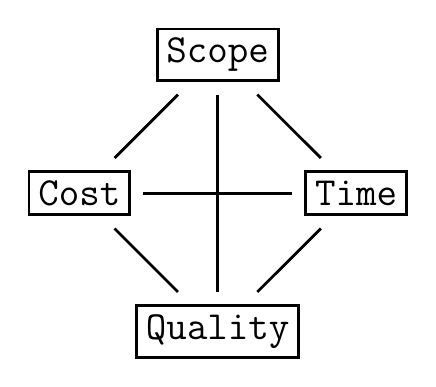
\begin{tikzpicture}[node distance=5em,
  every path/.style={draw=black, line width=.1em},
  every node/.style={font={\Large\ttfamily}, draw=black, rectangle, outer sep=.5em}]
\node[draw=none] (center) {};
\node[above of=center] (scope) {Scope};
\node[below of=center] (quality) {Quality};
\node[right of=center] (time) {Time};
\node[left of=center] (cost) {Cost};
\path (scope) -- (time);
\path (time) -- (cost);
\path (cost) -- (scope);
\path (quality) -- (time);
\path (quality) -- (cost);
\path (quality) -- (scope);
\end{tikzpicture}
}

\pmbaQuestion
  {ISO 9000 defines quality as ...}
  {the ultimate objective of any project}
  {the indicator of customer satisfaction}
  {the amount of defects that the customer experience in the product}
  {the degree to which a set of characteristics fulfil requirements}
  {iso}

\pmbaQuestion
  {The architect tells you that 15 bugs can't be fixed in current release and will be shipped to the customer. What do you say?}
  {``Cancel the release!''}
  {``Don't release until they are all fixed!''}
  {``Don't tell the customer, ship it anyway.''}
  {``How much trouble they may cause?''}
  {coq}

\pmbaQuestion
  {You just hired a ``QA Expert.'' What task you would give him?}
  {Help programmers make our app bug-free}
  {Test our mobile app and make sure it works well}
  {Find three bugs in our app}
  {Make sure every bug is in JIRA}
  {qa}

\pmbaQuestion
  {You want to increase \emph{quality of product}, which metric you would control first?}
  {Git commits per day}
  {Customer complaints per day}
  {CI failures per day}
  {New bugs per day}
  {qc}

\pmbaQuestion
  {You recruit an external team of testers, how would you pay them?}
  {\$100 per hour}
  {\$100 per feature they test}
  {\$100 per test case they execute}
  {\$100 per bug they find}
  {testers}

\pmbaQuestion
  {Customer complains that the quality is low: too many bugs in each new release. How can you find out the \emph{root cause}?}
  {Five Whys}
  {Plan-Do-Check-Act}
  {Six Sigma}
  {Fish-bone Analysis}
  {root-cause}

\pmbaQuestion
  {The biggest \emph{enemy} of quality is...}
  {Bureaucracy}
  {Bugs}
  {Negligence}
  {Enthusiasm}
  {ingredients}

\pmbaQuestion
  {There are four bugs reported, which one you would prioritize as more \emph{important} than others?}
  {A flow is missed in the Use Case}
  {A class has too many methods}
  {A unit test breaks the build}
  {A security loophole discovered in production server}
  {priorities}

\plush{
  \pptBanner{Homework:}
  ``\emph{Quality Management Plan} describes how quality policies will be implemented and how the project management team plans to meet the quality requirements set for the project''
  --- PMBOK5
}

\plush{
  \pptBanner{Read this:}
  \href{https://www.youtube.com/watch?v=jZitXMQaXvE}{Quality Assurance vs. Testing} at QAFest'19\par
  \href{https://www.yegor256.com/2022/07/05/safety-net.html}{Automated Tests Are the Safety Net that Saves You}\par
  \href{https://www.yegor256.com/2017/05/23/unlimited-number-of-bugs.html}{Any Program Has an Unlimited Number of Bugs} (2017)\par
  \href{https://www.yegor256.com/2015/09/10/testing-exit-criteria.html}{When Do You Stop Testing?} (2015)\par
  \href{https://www.yegor256.com/2014/08/22/art-of-software-testing.html}{The Art of Software Testing by Glenford Myers} (2014)\par
  \href{https://www.yegor256.com/2017/12/26/software-quality-formula.html}{The Formula for Software Quality} (2017)\par
}

\end{document}
